%**************************************************************************************
% License:
% CC BY-NC-SA 4.0 (http://creativecommons.org/licenses/by-nc-sa/4.0/)
%**************************************************************************************

\documentclass[notes]{beamer}

\mode<presentation> {

\usetheme{Madrid}

% Burnt orange
\definecolor{burntorange}{rgb}{0.8, 0.33, 0.0}
\colorlet{beamer@blendedblue}{burntorange}
% Pale yellow
\definecolor{paleyellow}{rgb}{1.0, 1.0, 0.953}
\setbeamercolor{background canvas}{bg=paleyellow}
% Secondary and tertiary palett
\setbeamercolor*{palette secondary}{use=structure,fg=white,bg=burntorange!80!black}
\setbeamercolor*{palette tertiary}{use=structure,fg=white,bg=burntorange!60!black}

% To remove the footer line in all slides uncomment this line
%\setbeamertemplate{footline}
% To replace the footer line in all slides with a simple slide count uncomment this line
%\setbeamertemplate{footline}[page number]

% To remove the navigation symbols from the bottom of all slides uncomment this line
%\setbeamertemplate{navigation symbols}{}
}

\usepackage{amsmath}
\usepackage{bm}
\usepackage{breqn}
\usepackage{graphicx} % for figures
\usepackage{subcaption} % for subplots 
\usepackage[labelsep=space,tableposition=top]{caption}
\renewcommand{\figurename}{Fig.} 
\usepackage{cleveref}
\usepackage{caption,subcaption}% http://ctan.org/pkg/{caption,subcaption}
\usepackage{booktabs} % Allows the use of \toprule, \midrule and \bottomrule in tables
\usepackage{multirow}

% To print 2 slides on a page
%\usepackage{handoutWithNotes}
%\pgfpagesuselayout{2 on 1}[border shrink=2mm]
%----------------------------------------------------------------------------------------
%	TITLE PAGE
%----------------------------------------------------------------------------------------
% The short title appears at the bottom of every slide, the full title is only on the title page
\title[CE394M: Constitutive Modeling]{CE394M: Constitutive Modeling} 
\author{Krishna Kumar} % name
\institute[UT Austin] % institution 
{
University of Texas at Austin \\
\medskip
\textit{
  \url{krishnak@utexas.edu}} % Your email address
}
\date{\today} % Date, can be changed to a custom date

\begin{document}

\begin{frame}
\titlepage % title page as the first slide
\end{frame}

\begin{frame}
 % Table of contents slide, comment this block out to remove it
 \frametitle{Overview}
  %Throughout your presentation, if you choose to use \section{} and \subsection{} 
  %commands, these %will automatically be printed on this slide as an overview 
 \tableofcontents
\end{frame}

%----------------------------------------------------------------------------------------
% slides
%----------------------------------------------------------------------------------------
\note{
	The objective of constitutive modelling is the determination of stiffness tensor $\mathbf{C}$, a relation between stress and strain tensors.

}
\section{Definition of stress and strain tensors}
%----------------------------------------------------------------------------------------
\begin{frame}
\frametitle{Stresses}
\mode<beamer>{
	\begin{figure}[ht]
	\centering
	\begin{subfigure}[b]{0.49\linewidth}
		\centering
		\includegraphics[width=\textwidth]{figs/stress-equilibrium.png}
	\end{subfigure}	
	\begin{subfigure}[b]{0.49\linewidth}
		\centering
		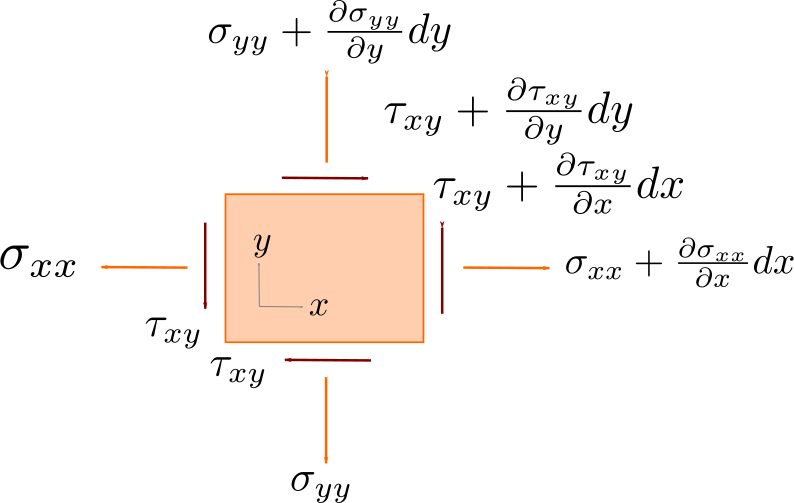
\includegraphics[width=0.85\textwidth]{figs/equilibrium-finished.pdf}
	\end{subfigure}%
\end{figure}
\begin{itemize}
	\item Stress state at a point is defined by $\sigma_{ij}$ in a frame of reference. 
	\item Equilibrium of moments require $sigma_{xz} = \sigma_{zx}, \dots$ etc.,
\end{itemize}
}
\mode<handout>{
	\begin{figure}[ht]
		\centering
		\begin{subfigure}[b]{0.49\linewidth}
			\centering
			\includegraphics[width=\textwidth]{figs/stress-equilibrium.png}
		\end{subfigure}	
		\begin{subfigure}[b]{0.49\linewidth}
			\centering
			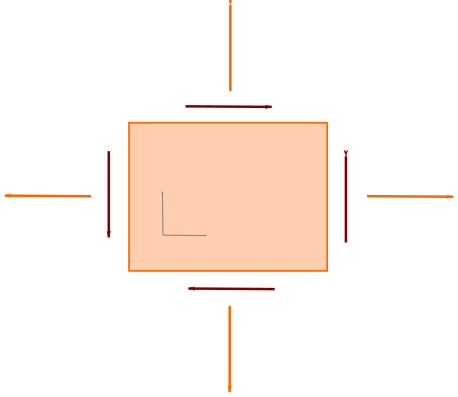
\includegraphics[width=0.85\textwidth]{figs/equilibrium.pdf}
		\end{subfigure}%
	\end{figure}
	\vspace{2cm}
}
\end{frame}
\note{
	\begin{itemize}
		\item $\sigma_{xz}$ stress acting on plane perpendicular to axis $x$ and in the direction of $z$
		\item $\sigma_{xx}$ stress acting on plane perpendicular to axis $x$ and in the direction of $x$
	\end{itemize}

}

%----------------------------------------------------------------------------------------
\begin{frame}
\frametitle{Stresses}
\noindent
\fboxsep=0pt
\noindent
\begin{minipage}[t]{0.59\linewidth}
	\mode<beamer>{	
		\begin{itemize}
			\item 9 components of the stress tensor.
			\item 6 stresses: $\sigma_{11}, \sigma_{22}, \sigma_{33}, \tau_{12}, \tau_{23}, \tau_{31}$.
			\item $\tau_{21} = -\tau_{12}, \tau_{32} = - \tau_{23}, \tau_{13} = - \tau_{31}$
			\item Compression is positive
			\item Shear stress, anti-clockwise is positive
			\item In order to write the components in a more concise way we can use the indices notation: $\sigma_{ij}$ (use $i = 1,2,3$ and $j = 1,2,3$)
			\item Correspondence from $x, y, z$ to $1, 2, 3$ (e.g., $\sigma_{11} = \sigma_{xx}, \sigma_{12} = \sigma_{xy}$)
		\end{itemize}
	}
\end{minipage}%
\hfill%
\begin{minipage}[t]{0.39\linewidth}
	\begin{figure}
		\includegraphics[width=\textwidth]{figs/stresses.png}
	\end{figure}
\end{minipage}	
\end{frame}

%----------------------------------------------------------------------------------------
\begin{frame}
\frametitle{Stress vector on a plane}
\begin{figure}[ht]
	\centering
	\includegraphics[width=0.7\textwidth]{figs/stress-vector-plane.png}
	\caption*{Stress vector on a plane normal to $\mathbf{\hat{n}}$ (Reddy., 2008)}
\end{figure}

If we denote by $\Delta (\mathbf{f\hat{n}})$ the force on a small area $\mathbf{\hat{n}}$ located at the position $x$, the stress vector can be defined:
\mode<beamer>{	
	\begin{equation*}
		\mathbf{t(\hat{n})} = \lim_{\Delta a \to 0} \frac{\Delta \mathbf{f(\hat{n})}}{\Delta a}
	\end{equation*}
Cauchy stress is the true stress, that is, stress in the deformed configuration.
}
\mode<handout>{	
	\vspace{2cm}
}
\end{frame}

%----------------------------------------------------------------------------------------
\begin{frame}
\frametitle{Cauchy stress tensor}
To establish the relationship between $\mathbf{t}$ and $\mathbf{\hat{n}}$ we now set up an infinitesimal
tetrahedron in Cartesian coordinates:
\begin{figure}[ht]
	\centering
	\includegraphics[width=0.4\textwidth]{figs/stress-tetrahedron.png}
	%\caption*{Tetrahedral element in Cartesian coordinates (Reddy., 2008)}
\end{figure}
If $\mathbf{-t}_1, \mathbf{-t}_2, \mathbf{-t}_3$ and $\mathbf{t}$ denote the stress vectors in the outward directions on the faces of the infinitesimal tetrahedron whose areas are $\Delta a_1, \Delta a_2, \Delta a_3$, and $\Delta a$, respectively. $\Delta v$ is the volume of the tetrahedron, $\rho$ the density, $f$ the body force per unit mass, and $\mathbf{a}$ the acceleration. 
\end{frame}

%----------------------------------------------------------------------------------------
\begin{frame}
\frametitle{Cauchy stress tensor}
we have by Newton's second law for the mass inside the tetrahedron:
\mode<beamer>{	
	\begin{equation*}
		\mathbf{t}\Delta a - \mathbf{t}_1 \Delta a_1
- \mathbf{t}_1 \Delta a_1 - \mathbf{t}_1 \Delta a_1 + \rho \Delta v \mathbf{f} = \rho \Delta v \mathbf{a}
	\end{equation*}
}
\mode<handout>{
	\vspace{1.5cm}
}

Since the total vector area of a closed surface is zero (gradient theorem):
\mode<beamer>{	
	\begin{equation*}
	\Delta a \mathbf{\hat{n}} - \Delta a_1 \mathbf{\hat{e}}_1 - \Delta a_2 \mathbf{\hat{e}}_2
	- \Delta a_3 \mathbf{\hat{e}}_3 = \mathbf{0}
	\end{equation*}
	\begin{equation*}
	\Delta a_1 =
	(\mathbf{\hat{n}}\cdot\mathbf{\hat{e}}_1) \Delta a, \quad 
	\Delta a_2 = (\mathbf{\hat{n}}\cdot\mathbf{\hat{e}}_2) \Delta a, \quad 
	\Delta a_3 = (\mathbf{\hat{n}}\cdot\mathbf{\hat{e}}_3) \Delta a. 
	\end{equation*}
}
\mode<handout>{
	\vspace{1.5cm}
}

The volume $\Delta v$ can be expressed as: \mode<beamer>{$\Delta v = (\Delta h / 3) \Delta a$}
where $\Delta h$ is the perpendicular distance from the origin to the slant face.
\mode<beamer>{	
	\begin{equation*}
	\mathbf{t} = 
	(\mathbf{\hat{n}}\cdot\mathbf{\hat{e}}_1) \mathbf{t}_1 +
	 (\mathbf{\hat{n}}\cdot\mathbf{\hat{e}}_2) \mathbf{t}_2 + 
	 (\mathbf{\hat{n}}\cdot\mathbf{\hat{e}}_3) \mathbf{t}_3 + \rho \frac{\Delta h}{3}(\mathbf{a - f})
	\end{equation*}
}
\mode<handout>{
	\vspace{1.5cm}
}
\end{frame}

%----------------------------------------------------------------------------------------
\begin{frame}
\frametitle{Cauchy stress tensor}
In the limit when the tetrahedron shrinks to a point $\Delta h \to 0$:
	\begin{equation*}
	\mathbf{t} = 
(\mathbf{\hat{n}}\cdot\mathbf{\hat{e}}_1) \mathbf{t}_1 +
(\mathbf{\hat{n}}\cdot\mathbf{\hat{e}}_2) \mathbf{t}_2 + 
(\mathbf{\hat{n}}\cdot\mathbf{\hat{e}}_3) \mathbf{t}_3 = (\mathbf{\hat{n}}\cdot\mathbf{\hat{e}}_i) \mathbf{t}_i
\end{equation*}
where the summation convention is used.
\mode<beamer>{	
	\begin{equation*}
	\mathbf{t} = 
\mathbf{\hat{n}}\cdot(\mathbf{\hat{e}}_1 \mathbf{t}_1 +
 \cdot\mathbf{\hat{e}}_2 \mathbf{t}_2 + 
\mathbf{\hat{e}}_3 \mathbf{t}_3).
	\end{equation*}
}
\mode<handout>{
	\vspace{1.5cm}
}

The terms in the parenthesis is the 
\textit{\textbf{stress tensor}} $\sigma$:
\begin{equation*}
	\sigma \equiv \mathbf{\hat{e}}_1 \mathbf{t}_1 +
\cdot\mathbf{\hat{e}}_2 \mathbf{t}_2 + 
\mathbf{\hat{e}}_3 \mathbf{t}_3
\end{equation*}
The stress tensor is a property of the medium that is independent of the $\mathbf{\hat{n}}$
\mode<beamer>{	
	\begin{equation*}
	\mathbf{t}(\mathbf{\hat{n}}) = 
\mathbf{\hat{n}}\sigma = \sigma^T \mathbf{\hat{n}}.
	\end{equation*}
}
\mode<handout>{
	\vspace{1.5cm}
}
The stress vector $\mathbf{t}$ represents the vectorial stress on a plane whose normal is $\mathbf{\hat{n}}$. $\sigma$ is the \textit{Cauchy stress tensor} defined to be the \textit{current force per unit deformed area}. In Cartesian component, the Cauchy formula is: $t_i = n_j \sigma_{ji}$.
\end{frame}

%----------------------------------------------------------------------------------------
\begin{frame}
\frametitle{Cauchy stress tensor}
\begin{figure}[ht]
	\centering
	\includegraphics[width=0.4\textwidth]{figs/cauchy-stress.png}
	\caption*{Wikipedia}
\end{figure}
\mode<beamer>{	
	The Cauchy stress tensor $\sigma$, which takes a directional unit vector $e$ as input and maps it to the stress vector $T(e)$, which is the force (per unit area) exerted by material on the negative side of the plane orthogonal to $e$ against the material on the positive side of the plane, thus expressing a relationship between these two vectors
}
\end{frame}

%----------------------------------------------------------------------------------------
\begin{frame}
\frametitle{Cauchy stress vs Piola-Kirchoff stress}
\begin{figure}[ht]
	\centering
	\includegraphics[width=\textwidth]{figs/cauchy-kirchoff-stress-tensor.png}
	\caption*{An introduction to continuum mechanics - J. N. Reddy (2008)}
\end{figure}
\mode<beamer>{
	\begin{itemize}
		\item The first Piola–Kirchhoff stress tensor, also referred to as the \textit{nominal stress tensor},
		or \textit{Lagrangian stress tensor}, gives the current force per unit undeformed area.
	\end{itemize}
}
\mode<handout>{
	\vspace{2cm}
}
\end{frame}
\end{document}